% PVK resources: https://polybox.ethz.ch/index.php/s/FQI5tkf1kabHnhB
% PW: SD2022
%
%
\documentclass[a4paper,10pt,landscape]{scrartcl}
\usepackage{algorithm}
\usepackage{algpseudocode}
\usepackage{multirow}
\usepackage{graphicx}
\usepackage{wrapfig}
\usepackage{tabularx}
\usepackage[table]{xcolor}
% \usepackage{svg}
% \usepackage{svg-extract}
% \svgsetup{clean=true}
\usepackage{scrlfile}
\PreventPackageFromLoading{svg}


% for a more readable preamble
% document setup
\usepackage[margin=3mm,landscape]{geometry} % margin = .. total={280mm,190 mm} % in geometry for defined size/ratio
\usepackage{multicol,multirow}
\usepackage[utf8]{inputenc} % not strictly necessary, but sets utf8

% enable colors
\usepackage{xcolor,color} % standard colors (blue, red, etc.https://www.namsu.de/Extra/pakete/Xcolor.html )

% multicol settings
\setlength{\premulticols}{1pt}
\setlength{\postmulticols}{1pt}
\setlength{\multicolsep}{1pt}
\setlength{\columnsep}{5pt}
\setlength{\columnseprule}{1pt}
\def\columnseprulecolor{\color{black}}

% language
\usepackage[english]{babel} %choose your language

% for images
\usepackage{graphicx}
\graphicspath{ {./images/} }

% Images combined with texts
\usepackage{wrapfig}

% some AsmTeX options
\usepackage{amscd, amsmath,amssymb}

% more fine control for lists
\usepackage{enumitem}

% multiple line comments and testing text
\usepackage{verbatim} % \begin{comment} \end{comment} 
\usepackage{blindtext} % inserts lorem ipsum like text

% hyperlinks (has to be after titlesec, else we get errors
\usepackage[colorlinks=true,citecolor=blue,linkcolor=blue]{hyperref}

% svg support
\usepackage[clean]{svg}
% colors
\usepackage{color,xcolor}
\definecolor{section}{HTML}{40916c}
\definecolor{subsection}{HTML}{52b788}
\definecolor{subsubsection}{HTML}{74c69d}
\definecolor{titletext}{RGB}{0,0,0}

% colored box for section
\setkomafont{section}{\mysection}
\newcommand{\mysection}[1]{%
    \setlength{\fboxsep}{0cm}%already boxed
    \colorbox{section}{%
        \begin{minipage}{\linewidth}%
            \vspace*{2pt}%Space before
            \hspace{2pt}%left indent
            #1
            \vspace*{2pt}%Space after
        \end{minipage}%
    }}
% colored box for subsection
\setkomafont{subsection}{\mysubsection}
\newcommand{\mysubsection}[1]{%
    \setlength{\fboxsep}{0cm}%already boxed
    \colorbox{subsection}{%
        \begin{minipage}{\linewidth}%
            \vspace*{2pt}%Space before
            \hspace{2pt}%left indent
            #1
            \vspace*{2pt}%Space after
        \end{minipage}%
    }}
% colored box for subsection
\setkomafont{subsubsection}{\mysubsubsection}
\newcommand{\mysubsubsection}[1]{%
    \setlength{\fboxsep}{0cm}%already boxed
    \colorbox{subsubsection}{%
        \begin{minipage}{\linewidth}%
            \vspace*{2pt}%Space before
            \hspace{2pt}%left indent
            #1
            \vspace*{2pt}%Space after
        \end{minipage}%
    }}

% decrease wasted space in title
\RedeclareSectionCommand[
  %runin=false,
  afterindent=false,
  beforeskip=.25\baselineskip,
  afterskip=.25\baselineskip]{section}
\RedeclareSectionCommand[
  %runin=false,
  afterindent=false,
  beforeskip=.25\baselineskip,
  afterskip=.25\baselineskip]{subsection}
\RedeclareSectionCommand[
  %runin=false,
  afterindent=false,
  beforeskip=.2\baselineskip,
  afterskip=.25\baselineskip]{subsubsection}
\RedeclareSectionCommand[
  runin=true,
  %afterindent=false,
  beforeskip=.25\baselineskip,
  afterskip=1em]{paragraph}
\RedeclareSectionCommand[
  runin=true,
  %afterindent=false,
  beforeskip=.5\baselineskip,
  afterskip=1em]{subparagraph}

% set the size of a section
\usepackage{parskip}
\setlength{\parindent}{0pt}
\setlength{\parskip}{0pt plus 0.5ex}

% un-comment to hide the section numbering
%\setcounter{secnumdepth}{0} 
%-----------------------------------------------------%
% for colours
\usepackage{color}
% from code expert "ce_"
\definecolor{ce_yellow}{HTML}{228B22}
\definecolor{ce_gray}{rgb}{0.459,0.443,0.369}
\definecolor{ce_lime}{rgb}{0.459,0.816,0.180}
\definecolor{ce_pink}{rgb}{0.976,0.149,0.447}
\definecolor{ce_cyan}{rgb}{0.40,0.851,0.937}
\definecolor{ce_violet}{rgb}{0.545,0.506,1.00}
\definecolor{ce_back}{rgb}{1,1,1}
\definecolor{ce_white}{rgb}{0.15,0.15,0.12}
%----------------------------------------------------%
% as close to CodeExpert as i could get it
\usepackage{listings}

\lstdefinestyle{CodeExpert}{
    language=C++,
    basicstyle=\ttfamily\linespread{0.8}\color{ce_white},
    numbers=none,
    aboveskip=0mm,
    belowskip=0mm,
    frame = none,
    numberstyle=\tiny\color{ce_grey},
    backgroundcolor = \color{ce_back},
    keywordstyle=\color{ce_cyan},
    commentstyle=\color{ce_gray},
    stringstyle=\color{ce_yellow},
    morecomment=[n][\color{ce_pink}]{\#}{\ },
    literate=
    *{./}{{{\color{ce_pink}./}}}2
    {.^}{{{\color{ce_pink}.\^{}}}}2
    {=}{{{\color{ce_pink}=}}}1
    {+}{{{\color{ce_pink}+}}}1
    {*}{{{\color{ce_pink}*}}}1
    {-}{{{\color{ce_pink}-}}}1
    {&}{{{\color{ce_pink}&}}}1
    {<<}{{{\color{ce_pink}<<}}}2
    {>>}{{{\color{ce_pink}>>}}}2
    {<}{{{\color{ce_pink}<}}}1
    {>}{{{\color{ce_pink}>}}}1
    {->}{{{\color{ce_pink}->}}}2
    {1}{{{\color{ce_violet}1}}}1
    {2}{{{\color{ce_violet}2}}}1
    {3}{{{\color{ce_violet}3}}}1
    {4}{{{\color{ce_violet}4}}}1
    {5}{{{\color{ce_violet}5}}}1
    {6}{{{\color{ce_violet}6}}}1
    {7}{{{\color{ce_violet}7}}}1
    {8}{{{\color{ce_violet}8}}}1
    {9}{{{\color{ce_violet}9}}}1
    {0}{{{\color{ce_violet}0}}}1
    {this}{{{\color{ce_lime}this}}}1
    {if}{{{\color{ce_pink}if}}}1
    {do}{{{\color{ce_pink}do}}}1
    {for}{{{\color{ce_pink}for}}}1
    {else}{{{\color{ce_pink}else}}}1
    {then}{{{\color{ce_pink}then}}}1
    {break}{{{\color{ce_pink}break}}}1
    {continue}{{{\color{ce_pink}continue}}}1
    {public}{{{\color{ce_pink}public}}}1
    {private}{{{\color{ce_pink}private}}}1
    {while}{{{\color{ce_pink}while}}}1
    {continue}{{{\color{ce_pink}continue}}}1
    {nullptr}{{{\color{ce_violet}nullptr}}}1
    {NULL}{{{\color{ce_violet}NULL}}}1,
}

\lstset%
    {
    basicstyle=\ttfamily,
    frame=tb,
    aboveskip=1mm,
    belowskip=1mm,
    showstringspaces=true,
    columns=flexible,
    breaklines=true,
    breakatwhitespace=true,
    tabsize=2,
}
%Mathematik-Pakete
\usepackage{amsmath, amstext, amssymb, mathtools, esint, polynom}
\usepackage{bm}
\allowdisplaybreaks %Seitenumbruch in align-Umgebung erlauben
%

%Definition der Umgebung "example"
\newenvironment {example}
				{\begin{itshape} \begin{small}}
				{\end{small} \end{itshape}}
%				
%Definition der Umgebung "annotation"		
\newenvironment {annotation}[1]
				{\begin{itshape} \begin{small} \textbf{#1} \begin{itemize}}
				{\end{itemize} \end{small} \end{itshape}}
%				
%Definition der Umgebung "eq"
\newenvironment {eq}
				{\begin{equation*}}
				{\end{equation*}}
%
% Don't know what this does
\providecommand{\diff}{\mathop{} \! \mathrm{d}}
\DeclareMathOperator{\rot}{rot}
\DeclareMathOperator{\divg}{div}
% -------------------------------------------
\title{PSA Summary}
\subtitle{HS24 ETH Zurich}
\author{Carl von Holly-P.}
% \date{\today}
%
\begin{document}
\begin{multicols*}{3}
%
\maketitle
\section{Basics}
resistance and reactance:
$z=r+jx=\frac{1}{y} = \frac{1}{g + jb}$ \\
conductance and susceptance:
$g=\frac{r}{r^2 + x^2}$ \\
$b=\frac{x}{r^2 + x^2}$ \\
per unit: $r=r^{pu}\cdot r_{base}\quad\left[\mathrm{p.u.}\right]\cdot\left[\mathrm{\frac{\Omega}{p.u.}}\right]$
\section{Components}
\subsection{Transmission line}
$\underline{I}_{k m}=\left(a_{k m}^2 \underline{E}_k-t_{k m}^* t_{m k} \underline{E}_m\right) y_{k m}+y_{k m}^{S h} a_{k m}^2 \underline{E}_k$

\subsection{Phase shifting transformers}
\begin{figure}[H]
    \centering
    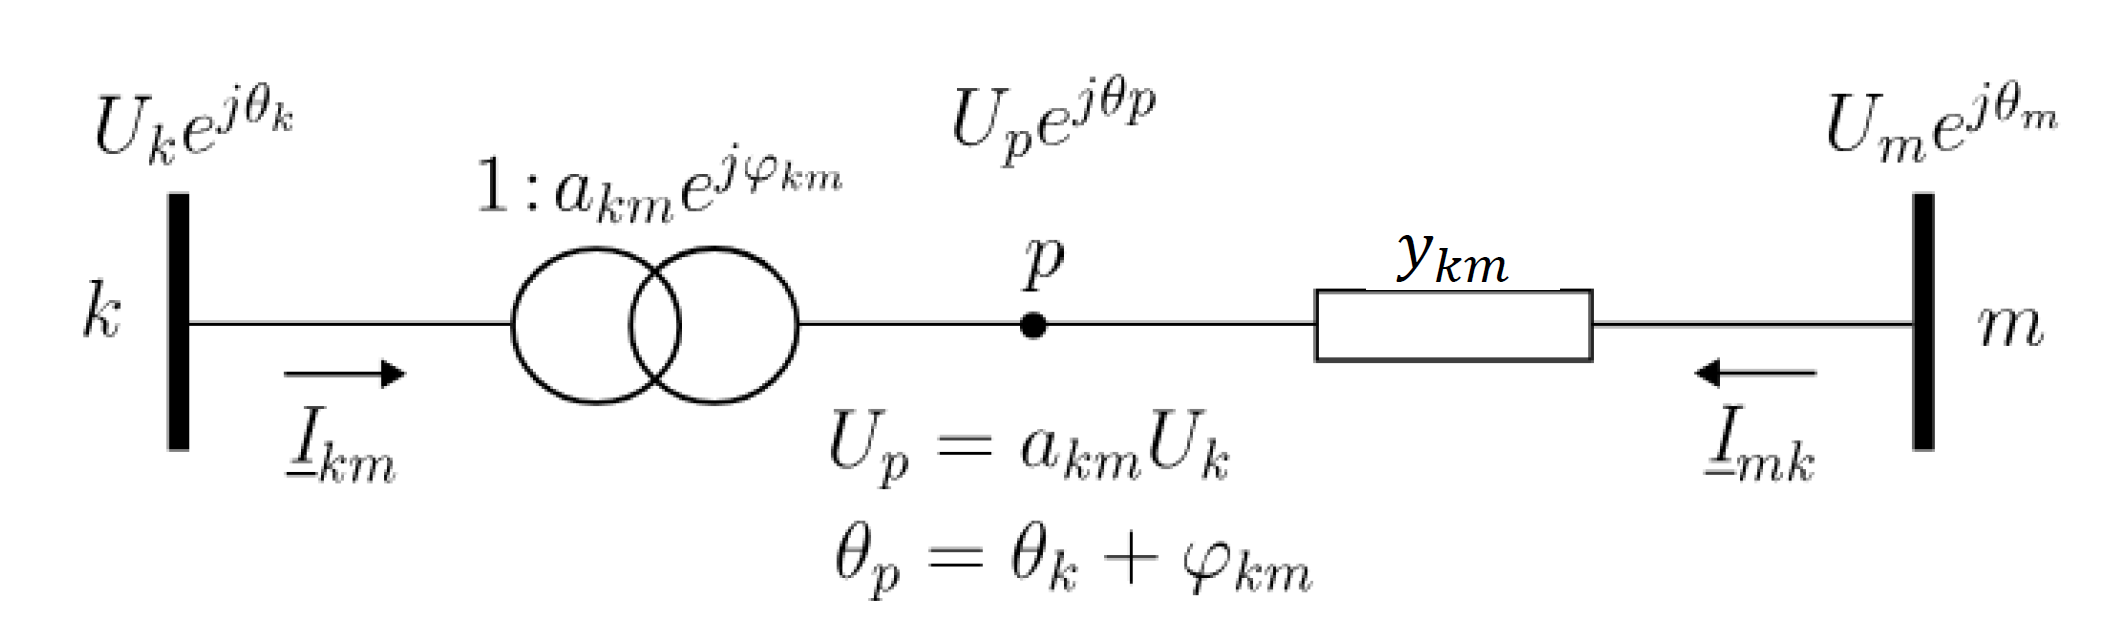
\includegraphics[width=\linewidth]{src/image.png}
\end{figure}
$\binom{\underline{I}_{k m}}{\underline{I}_{m k}}=\left(\begin{array}{cc}a_{k m}^2 y_{k m} & -t_{k m}^* y_{k m} \\ -t_{k m} y_{k m} & y_{k m}\end{array}\right)\binom{\underline{E}_k}{\underline{E}_m}$ \\
$\begin{aligned} P_{k m} & =a_{k m}^2 U_k^2 g_{k m}-a_{k m} U_k U_m g_{k m} \cos \left(\theta_{k m}+\varphi_{k m}\right) \\ & -a_{k m} U_k U_m b_{k m} \sin \left(\theta_{k m}+\varphi_{k m}\right)\end{aligned}$
$\begin{aligned} Q_{k m} & =-a_{k m}^2 U_k^2 b_{k m}+a_{k m} U_k U_m b_{k m} \cos \left(\theta_{k m}+\varphi_{k m}\right) \\ & -a_{k m} U_k U_m g_{k m} \sin \left(\theta_{k m}+\varphi_{k m}\right)\end{aligned}$ \\
where $\theta_{km}=\theta_k-\theta_m$ the voltage angle difference, $t_{km}=a_{km}e^{j\varphi_{km}}$ the transformer model, $\varphi_{km}$ the phase shift.


\subsection{Unified Branch Model}
idea: combine all devices in one model. \\
Transmission line: $a_{km}=a_{mk}=1$, $\varphi_{km}=\varphi_{mk}=0$. \\
Transformers: $y^{sh}_{km}=y^{sh}_{mk}=0$, $a_{mk}=1$, $\varphi_{mk}=0$.
\begin{figure}[H]
    \centering
    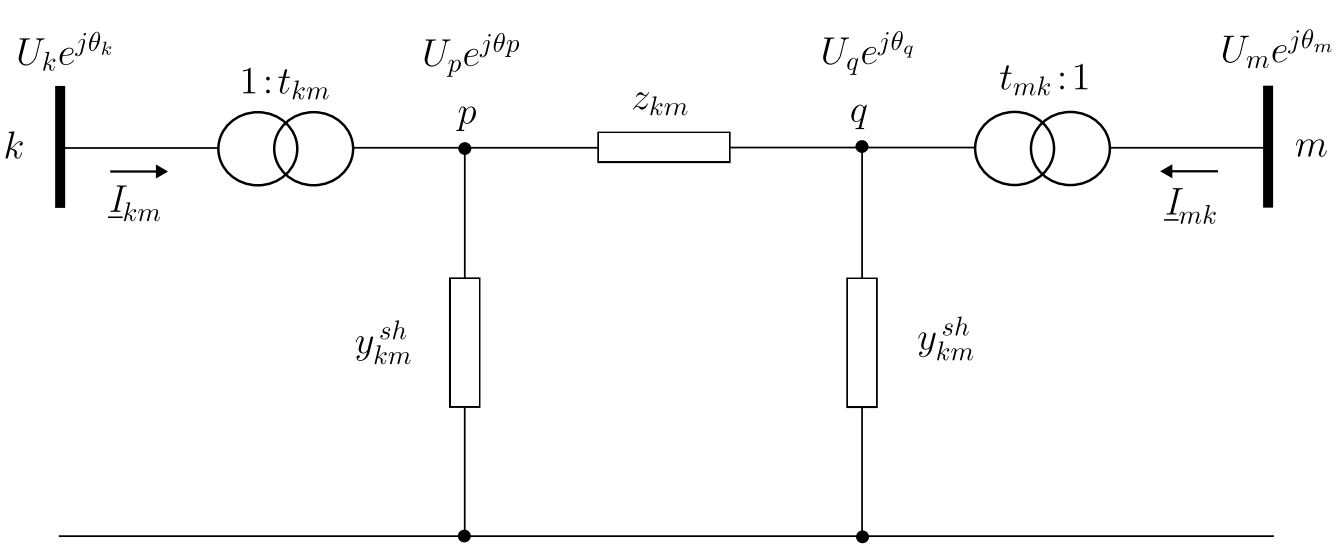
\includegraphics[width=1\linewidth]{src/ubm.png}
\end{figure}
$\binom{\underline{I}_{k m}}{\underline{I}_{m k}}=\left(\begin{array}{cc}a_{k m}^2\left(y_{k m}+y_{k m}^{s h}\right) & -t_{k m}^* t_{m k} y_{k m} \\ -t_{m k}^* t_{k m} y_{k m} & a_{m k}^2\left(y_{k m}+y_{k m}^{s h}\right)\end{array}\right)\binom{\underline{E}_k}{\underline{E}_m}$ \\
$\begin{aligned} P_{k m} & =\left(a_{k m} U_k\right)^2 g_{k m} \\ & -\left(a_{k m} U_k\right)\left(a_{m k} U_m\right) g_{k m} \cos \left(\theta_{k m}+\varphi_{k m}-\varphi_{m k}\right) \\ & -\left(a_{k m} U_k\right)\left(a_{m k} U_m\right) b_{k m} \sin \left(\theta_{k m}+\varphi_{k m}-\varphi_{m k}\right)\end{aligned}$ \\
$\begin{aligned} Q_{k m} & =-\left(a_{k m} U_k\right)^2\left(b_{k m}+b_{k m}^{s h}\right) \\ & +\left(a_{k m} U_k\right)\left(a_{m k} U_m\right) b_{k m} \cos \left(\theta_{k m}+\varphi_{k m}-\varphi_{m k}\right) \\ & -\left(a_{k m} U_k\right)\left(a_{m k} U_m\right) g_{k m} \sin \left(\theta_{k m}+\varphi_{k m}-\varphi_{m k}\right)\end{aligned}$


\subsection{shunt elements}
$I_k^{sh}=-y_k^{sh}E_k$ (meaning positive current for current \textit{into} bus $k$)

\subsection{loads}
Assume load active \& reactive power is constant.
\subsection{generators}
\subsubsection{capability curve}
$S_g=P_g + jQ_g$ is limited
\begin{itemize}
    \item in $P_{g,max}$ by stator current heating limit (max. losses in armature $R_t|I_t|^2$
    \item in $Q_{g,max}$ by field current heating limit
    \item in $Q_{g,min}$ by stator end region heating limit (eddy currents leading to heat)
\end{itemize}

\subsection{admittance matrix}
nodal admittance matrix: $\mathbf{Y=G+jB}\Rightarrow\mathbf{I=YE}$ \\
with elements
$Y_{km} = -t_{km}^*t_{mk}y_{km}$ \\
$Y_{kk} = y_k^{sh}+\underset{m\in\Omega_k}{\sum}a_{km}^2(y_{km}^{sh} + y_{km})$ \\
characteristics: \textit{sparse} and generally \textit{symmetric} (not in case of phase-shifting-trafo)

\section{Power Flow Computation}
\subsection{Bus Types}
variables: $P_k,Q_k,U_k,\theta_k$ (redundancy: 2 variables)

\begin{table}[H]
    \centering
    \begin{tabular}{c|c|c|c|c}
         Bus type&  a.k.a.& known's & equal. constr. & \\ \hline
         slack&  & $U_k,\theta_k=0$ & $U=$ const. & \\
         PQ&  load& $P_k,Q_k$ & $P,Q$ balance & \\
         PU&  gen.& $P_k,Q_k$ & $P$ balance, $U=$ const. & \\
    \end{tabular}
\end{table}

\subsection{DC Power Flow}
assumptions:
\begin{itemize}
    \item $|U_{bus}|=1$ at all buses
    \item small $\theta_{km}\Rightarrow \cos(\theta_{km})\approx1, \sin(\theta_{km})\approx \theta$
    \item lossless transmission lines \& power transformers
    \item neglect shunt elements
\end{itemize}
equations for tr.-line, in-phase-trafo, phase shifter:
$$P_{km}=\frac{\theta_{km}}{x_{km}} \quad P_{km}=\frac{\theta_{km}}{x_{km}/a_{km}} \quad P_{km}=\frac{\theta_{km}+\varphi_{km}}{x_{km}}$$
\subsubsection{DC Load Flow}
$$P_k=P_{G_{k}}-P_{L_{k}} = \underset{m\in\Omega_k}{\sum}\frac{\theta_k-\theta_m}{x_{km}}=B_{kk}'\theta_k + \underset{m\in\Omega_k}{\sum}B_{km}'\theta_m$$
$$\Rightarrow \mathbf{P=B'\theta}$$
Row $i$ may have to be deleted as $\theta_i=0$ is slack/reference bus. \\
With $\mathbf{P}$ vector of net injections, $\mathbf{B'}$ nodal admittance matrix. If there are phase shifting transformers: $\mathbf{P=B'\theta-P_{pst}}$

\subsection{Gauss(-Seidel) approach}







\section{Fault analysis}
Why do we care? Scale circuit breakers to correct size.

\subsection{Superposition technique}


\end{multicols*}
\end{document}